% fixture: tikz/nodes
% tier: T3
% engine: document
% specials: compare
% covers: named nodes (rectangle and circle, drawn, filled, rounded corners, minimum height, inner sep) with styles from \tikzset, positioning's right=of, below=of and above=… of with node distance, lines between nodes ending on their borders, an anchor (in.south), -| and |- to and from nodes, labels on lines, the nodes' text in the document's fonts (\textbf, \small around \tikz)
% issue: #320
\documentclass{article}
\usepackage{tikz}
\usetikzlibrary{positioning,arrows.meta}
\tikzset{block/.style={draw, fill=blue!10, rounded corners=2pt, minimum height=8mm}}
\begin{document}
A flow of named nodes, in a figure:
\begin{figure}[h]
\centering
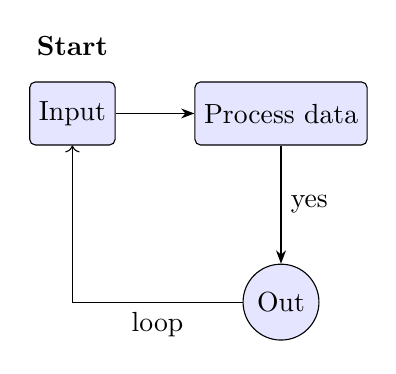
\begin{tikzpicture}[node distance=1.5cm and 1cm]
  \node[block] (in) {Input};
  \node[block, right=of in] (proc) {Process data};
  \node[block, below=of proc, circle] (out) {Out};
  \node[above=2mm of in] {\textbf{Start}};
  \draw[-Stealth] (in) -- (proc);
  \draw[-Stealth] (proc) -- node[right] {yes} (out);
  \draw[->, dashed] (out) -| node[near start, below] {loop} (in);
  \draw (in.south) |- (out.west);
\end{tikzpicture}
\caption{Nodes and lines between them}
\end{figure}
Inline, \tikz \node[draw, inner sep=1pt] {x}; and {\small a smaller
\tikz \node[draw] {small}; node} in a line of text.
\end{document}
